\section{Greedy Algorithm: Optimal Satellite Observation Scheduling}

\subsection{Real-World Problem Identification (10 pts)}
In satellite operations and space systems engineering, Earth-observing satellites in Low Earth Orbit (LEO) carry specialized optical and synthetic-aperture radar (SAR) payloads. Ground stations and scientific agencies submit requests to image specific terrestrial regions. Due to orbital dynamics and satellite velocity, each target ground location is visible only during a strict visibility window $[s_i, f_i)$, where $s_i$ denotes the acquisition start epoch and $f_i$ denotes the acquisition completion epoch.

The onboard imaging instrument can capture only one observation at a time; slewing the payload and operating sensors concurrently during overlapping windows is physically impossible. Therefore, satellite mission operations must schedule the maximum number of feasible observation requests within a single orbit pass without temporal conflict.

\subsection{Mathematical Abstraction (5 pts)}
We abstract this operational scenario as the \textit{Interval Scheduling Problem} over ground sets.
\begin{definition}[Interval Ground Set and Compatibility]
Let $\mathcal{I} = \{I_1, I_2, \dots, I_n\}$ be a set of $n$ requests. Each request is modeled as a half-open real interval:
\begin{equation}
I_i = [s_i, f_i) \subset \mathbb{R}, \quad \text{with } s_i < f_i.
\end{equation}
Two intervals $I_i, I_j \in \mathcal{I}$ ($i \neq j$) are mutually compatible if and only if their intersection is empty:
\begin{equation}
I_i \cap I_j = \emptyset \iff (f_i \le s_j) \lor (f_j \le s_i).
\end{equation}
A subset $S \subseteq \mathcal{I}$ is mutually compatible (an independent set) if all pairs in $S$ are pairwise compatible.
\end{definition}

\textbf{Optimization Objective:} Find a subset $S^* \subseteq \mathcal{I}$ such that $S^*$ is pairwise compatible and $|S^*| = \max \{ |S| : S \subseteq \mathcal{I} \text{ is compatible} \}$.

\subsection{Algorithmic Solution (10 pts)}
The greedy strategy selects intervals based on the \textit{Earliest Finish Time} (EFT) rule.

\begin{algorithm}[H]
\caption{Optimal Interval Scheduling (Greedy EFT)}
\label{alg:greedy_interval}
\begin{algorithmic}[1]
\REQUIRE Set of intervals $\mathcal{I} = \{I_1, \dots, I_n\}$ with $I_i = [s_i, f_i)$
\ENSURE Maximum cardinality compatible subset $S \subseteq \mathcal{I}$
\STATE Sort $\mathcal{I}$ in non-decreasing order of finish times such that $f_1 \le f_2 \le \dots \le f_n$.
\STATE Initialize $S \leftarrow \emptyset$
\STATE Initialize $f_{\text{last}} \leftarrow -\infty$
\FOR{$i = 1$ \TO $n$}
    \IF{$s_i \ge f_{\text{last}}$}
        \STATE $S \leftarrow S \cup \{I_i\}$
        \STATE $f_{\text{last}} \leftarrow f_i$
    \ENDIF
\ENDFOR
\RETURN $S$
\end{algorithmic}
\end{algorithm}

\subsection{Running Time Analysis (5 pts)}
The asymptotic runtime of Algorithm~\ref{alg:greedy_interval} is dominated by the initial sorting stage:
\begin{enumerate}
    \item \textbf{Sorting Stage:} Sorting $n$ intervals by finish time $f_i$ requires $\mathcal{O}(n \log n)$ comparisons using merge sort or heapsort.
    \item \textbf{Greedy Selection Pass:} The single linear scan processes each interval in $\mathcal{O}(1)$ time by evaluating the scalar condition $s_i \ge f_{\text{last}}$ and updating $f_{\text{last}}$. Across all $n$ elements, this phase runs in $\mathcal{O}(n)$ time.
    \item \textbf{Space Complexity:} The algorithm requires $\mathcal{O}(n)$ auxiliary storage for the sorted list and output set.
\end{enumerate}
Hence, total execution time is $\mathcal{O}(n \log n) + \mathcal{O}(n) = \mathcal{O}(n \log n)$.

\subsection{Proof of Correctness (10 pts)}
We prove the optimality of Algorithm~\ref{alg:greedy_interval} using a formal ``Greedy Stays Ahead'' inductive exchange argument.

\begin{theorem}
The set $S$ produced by Algorithm~\ref{alg:greedy_interval} has maximum cardinality among all mutually compatible subsets of $\mathcal{I}$.
\end{theorem}

\begin{proof}
Let $S = \{i_1, i_2, \dots, i_k\}$ be the ordered sequence of intervals selected by the greedy algorithm, where $f(i_1) \le f(i_2) \le \dots \le f(i_k)$.
Let $\mathcal{O} = \{j_1, j_2, \dots, j_m\}$ be any optimal compatible schedule ordered by finish time, with $f(j_1) \le f(j_2) \le \dots \le f(j_m)$. We aim to show that $k = m$.

\textbf{Lemma 1 (Greedy Stays Ahead):} For every $r \le k$, $f(i_r) \le f(j_r)$.
\begin{itemize}
    \item \textit{Base case ($r=1$):} The greedy algorithm selects $i_1$ as the interval with the earliest finish time among all available requests in $\mathcal{I}$. Therefore, $f(i_1) \le f(j_1)$.
    \item \textit{Inductive step:} Assume $f(i_{r-1}) \le f(j_{r-1})$ for some $r > 1$. Since $\mathcal{O}$ is compatible, interval $j_r$ starts after $j_{r-1}$ finishes, meaning $s(j_r) \ge f(j_{r-1})$. By the inductive hypothesis, $f(j_{r-1}) \ge f(i_{r-1})$, which implies $s(j_r) \ge f(i_{r-1})$. Thus, interval $j_r$ is compatible with the first $r-1$ greedy selections and was an eligible candidate when greedy selected interval $i_r$. Because greedy selects an eligible interval with minimum finish time, it follows that $f(i_r) \le f(j_r)$.
\end{itemize}
By induction, Lemma 1 holds for all $r \in \{1, \dots, k\}$.

Now assume for contradiction that $k < m$. By Lemma 1, $f(i_k) \le f(j_k)$. Since $m > k$, there exists an interval $j_{k+1} \in \mathcal{O}$. Since $\mathcal{O}$ is compatible, $s(j_{k+1}) \ge f(j_k) \ge f(i_k)$. Therefore, $j_{k+1}$ starts after $i_k$ finishes, meaning $j_{k+1}$ was compatible with all intervals in $S$. The greedy loop terminates only when no compatible intervals remain, contradicting the termination condition. Thus, $k \ge m$. Because $\mathcal{O}$ is optimal, $k \le m$. Hence $k = m$, proving that greedy produces an optimal schedule.
\end{proof}

\subsection{Problem Domain Translation (5 pts)}
In the operational context of satellite ground command:
\begin{itemize}
    \item \textbf{Sorting by Finish Time:} Mission planning sorts prospective target imagery requests by the exact timestamp when the target ground region leaves the field of view of the sensor.
    \item \textbf{Greedy Choice Property:} By always scheduling the acquisition that concludes earliest, the satellite payload operator frees up the imaging sensor as early as possible in the orbit pass, maximizing remaining orbital time for future acquisitions.
    \item \textbf{Compatibility Check:} The algorithm evaluates if the satellite can point its sensors at the next prospective ground target without requiring backward travel in time or conflicting with ongoing data capture ($s_i \ge f_{\text{last}}$).
\end{itemize}

\subsection{Implementation and Empirical Verification (5 pts)}
We implemented Algorithm~\ref{alg:greedy_interval} in Python and evaluated empirical runtime scaling across request workloads spanning $n \in [10^2, 2.5 \times 10^5]$. At each scale, random intervals were sampled uniformly over a continuous temporal mission horizon across five independent trials. Figure~\ref{fig:greedy_runtime} illustrates the measured mean runtime alongside the non-linear least-squares fitted curve $t(n) = c \cdot n \log_2 n$ with scaling constant $c \approx 1.521 \times 10^{-8}$. The coefficient of determination ($R^2 = 0.9883$) demonstrates precise agreement between empirical performance and the theoretical bound.

\begin{figure}[htbp]
\centering
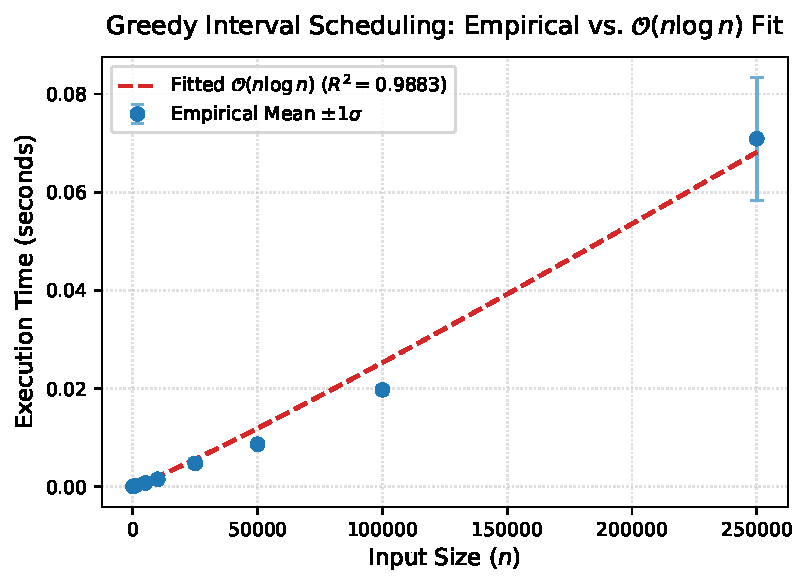
\includegraphics[width=\linewidth]{figures/greedy_runtime.pdf}
\caption{Empirical wall-clock runtime vs. theoretical $\mathcal{O}(n \log n)$ prediction for greedy interval scheduling across $n \in [10^2, 2.5 \times 10^5]$ requests ($R^2 = 0.9883$).}
\label{fig:greedy_runtime}
\end{figure}

